\documentclass[12pt, a4paper]{article}

\usepackage{enumerate}
\usepackage[top=5em, bottom=5em, left=5em, right=5em]{geometry}
\usepackage{graphicx}

\setlength\parskip{1em}
\setlength\parindent{0em}

\title{Assignment 3}

\author{Hendrik Werner s4549775}

\begin{document}
\maketitle

\section{} %1
\begin{enumerate}[a]
	\item %a
	\begin{tabular}{|c|c|c|}
		\hline
		Datagram & Source & Destination\\\hline
		1 & 10.0.1.13:3366 & 128.119.164.189:80\\
		2 & 135.122.204.209:10 & 128.119.164.189:80\\
		3 & 128.119.164.189:80 & 135.122.204.209:10\\
		4 & 128.119.164.189:80 & 10.0.1.13:3366\\
		\hline
	\end{tabular}

	\begin{tabular}{|c|c|c|c|}
		\hline
		\multicolumn{2}{|c|}{WAN Side} & \multicolumn{2}{|c|}{LAN Side}\\\hline
		IP & Port & IP & Port\\\hline
		135.122.204.209 & 10 & 10.0.1.13 & 3366\\
		\hline
	\end{tabular}

	\item %b
	The NAT router receives a packet with some destination IP and port. It then looks up this address in its NAT table to get the LAN side IP and port this address corresponds to. The packet's destination address is replaced by the NAT with the new LAN side destination address, the new checksum is calculated and set, and the packet is sent to the LAN.

	\item %c
	The destination and source fields are part of the checksum so the checksum needs to be recalculated if any of these change as mentioned in (b).

\end{enumerate}

\section{} %2
\begin{enumerate}[a]
	\item %a
	Every router needs to be able to communicate with every other router for the subnets to be connected. Every router has 4 interfaces and we have 3 routers so this makes 12 interfaces in total.

	If we assume that the routers can use routing protocols it is sufficient if there exists a path between two routers for them to be able to communicate and no direct connection is required. We use 2 interfaces to connect two routers (one interface for each of them). Concordantly we need $2 * 2 = 4$ of our 12 interfaces to connect the routers to each other.

	This leaves us with 8 interfaces that can be connected to subnets so 8 subnets can be connected, one to each interface.

	\item %b
	We can only have a resolution of powers of two. $90 < 2^7, 60 < 2^6, 12 < 2^6$ so we can serve all interfaces with 7 and 6 bits of freedom respectively thus giving us these possible addresses:

	\begin{tabular}{|c|c|c|}
		\hline
		Subnet & IP & Nr of addresses\\\hline
		1 & 223.1.17.0/26 & 64\\
		2 & 223.1.17.128/25 & 128\\
		3 & 223.1.17.64/26 & 64\\
		\hline
	\end{tabular}

\end{enumerate}

\section{} %3
\begin{enumerate}[1]
	\item %1
	C

	\item %2
	A, D

	\item %3
	C

	\item %4
	B, D

	\item %5
	Interface $I_1$ will be used because the path to x is shorter.

	\item %6
	When the connection between 4a and 2c is made the new shortest path to x goes through 1b so this time $I_2$ will have the shortest path and is concordantly used.

	\item %7
	In hot-potato routing each router tries to forward packages to another routers as fast as possible and does not hold onto anything. There is no package buffer but each packet is immediately forwarded upon being received. (That is where the name comes from: You do not want to hold onto a hot potato somebody threw your way.)
\end{enumerate}

\section{} %4
The lab files are provided in the folder zebraLab which is provided in the zip file with this pdf. Here is a screenshot of the VMs in action, pinging each other in a circle:

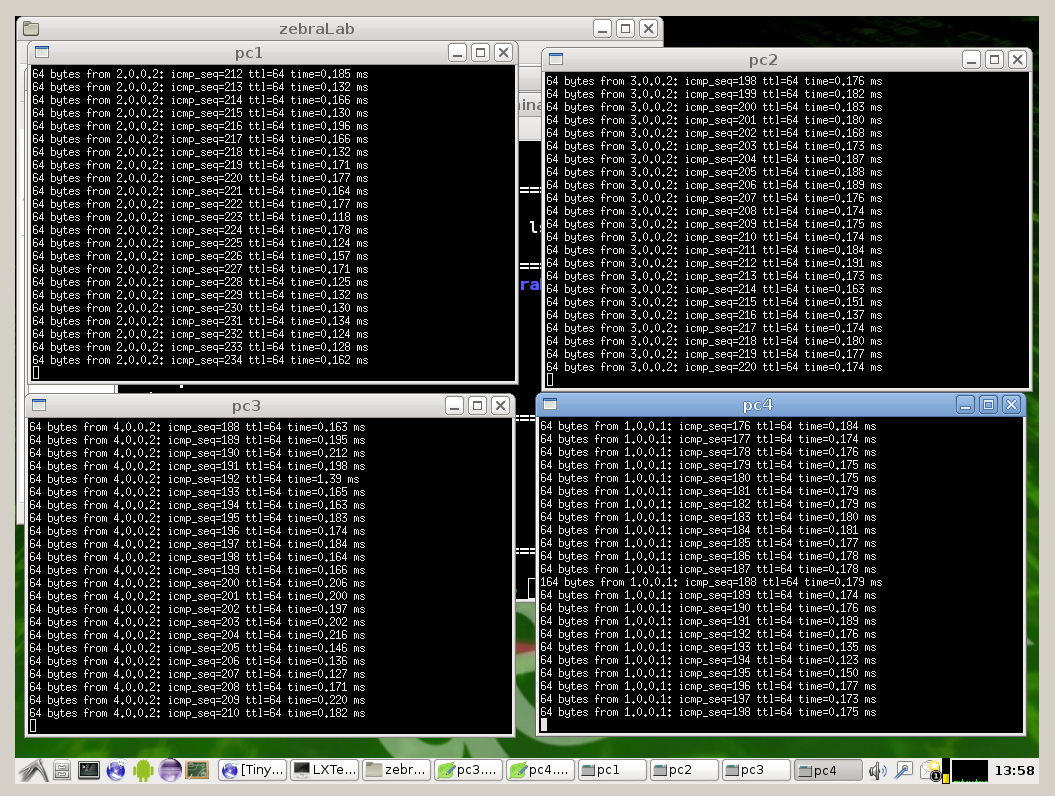
\includegraphics[width=\linewidth]{screenshots/netkit}

\section{} %5
\begin{enumerate}[1]
	\item %a
	IPv4 uses variable length headers while IPv6 has a fixed header size. IPv6 is much simpler than IPv4 and has 128 bit addresses compared to IPv4's 32 bit address space.

	\begin{tabular}{|p{18em}|c|c|}
		\hline
		\textbf{Description} & \multicolumn{2}{|c|}{\textbf{Field}}\\\hline
		& \textbf{IPv4} & \textbf{IPv6}\\\hline
		Version of the protocol & Version & Version\\\hline
		Length of the header & IHL &\\\hline
		Type of the service & DSCP & Traffic Class\\\hline
		Congestion Notification (IPv6 uses only the 2 least significant bits of the "Traffic Class" field for this) & ECN & Traffic Class\\\hline
		Length of the Content (for IPv4 this includes the header, which does not have a fixed site, for IPv6 it just includes the payload) & Total Length & Payload Length\\\hline
		Identification of groups of fragments (IPv6 does not include fragmentation) & Identification &\\\hline
		Flags to control fragmentation & Flags &\\\hline
		Fragmentation offset & Fragmentation Offset &\\\hline
		Remaining Hops until the packet is discarded (each router on the way decrements this number by 1) & TTL & Hop Limit\\\hline
		Protocol used in the datagram & Protocol &\\\hline
		Header Checksum (Because the TTL field is considered when calculating this checksum it is basically useless as it changes on every hop.) & Header Checksum &\\\hline
		Source Address (origin of the packet) & Source Address & Source Address\\\hline
		Destination Address () & Destination Address & Destination Address\\\hline
		Additional Options enabled via IHL & Options &\\\hline
		Flow Label used to maintain the sequential flow of packets && Flow Label\\\hline
	\end{tabular}

	\item %b
	Both IPv4 and IPv6 are Network Layer protocols so you could argue that it is misleading to say that IPv4 tunnels are treated as Link Layer protocols. But on the other hand each Layer uses the Layer below it as a black box and layers are separated (at least that's how it should be). Therefore you could say that IPv6 treats IPv4 tunnels as the new layer down which would be the Link Layer.

	I think it is not really false to say that but may be misleading so I wouldn't do that.
\end{enumerate}

\end{document}
